\documentclass[12pt]{article}
\usepackage{amsmath}
\usepackage{graphicx}
\usepackage{fullpage}
\usepackage{algorithm}
\usepackage{algorithmicx}
\usepackage[noend]{algpseudocode}
\usepackage{xcolor}

\title{Assignment 3 Solutions}
\author{COMP 3804, Fall 2018 \\
	Michael Kuang 101000485}
\date{November 19, 2018}
\begin{document}
\maketitle

\section{Guidelines}
General guidelines are as follows:
\begin{enumerate}
\item Since we are only accepting assignments via CU-Learn, no late submissions will be entertained after the cut-off time \& date. 

\item Please write clearly and answer questions precisely.  It is your responsibility to ensure that what is uploaded is clearly readable. If we can't read, we can't mark!


\item Please cite all the references (including web-sites, names of friends,
etc.) which you used/consulted as the source of information for each of
the questions. 


\item All questions/problems carry equal marks. 

\item When a question asks you to design an algorithm - it {\bf requires} you to 
\begin{enumerate}
\item Clearly spell out the {\bf steps}  of your algorithm in pseudo code.
\item {\bf Prove} that your algorithm is correct 
\item {\bf Analyze} the running time. 
\end{enumerate}

\item You can assume that a graph  $G=(V,E)$ uses adjacency list representation. 

\end{enumerate}

\newpage

\section{Problems}

\begin{enumerate}

\item \color{blue}Find strongly connected components of the graph in the Figure.

\color{black}
\textbf{Solution}\\
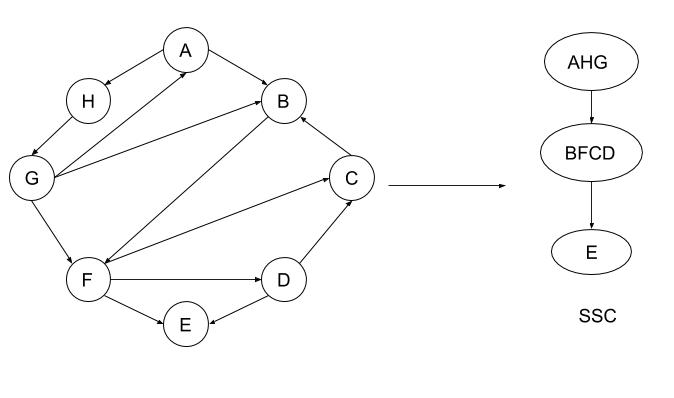
\includegraphics[scale=0.5]{q1}

% Question 2
\item \color{blue} Let $G=(V,E)$ be a directed graph. We say that $G$ is {\em semi-connected} if for every pair of distinct vertices $u,v\in V$,  we have that there is a directed path from $u$ to $v$ or there is a directed path from $v$ to $u$ in $G$.  Given $G$ in the adjacency list representation, design an algorithm running in $O(|V|+|E|)$ time to determine whether $G$ is semi-connected. Note that this is similar to the question which we had in the mid-term, where we needed to check whether a directed acyclic graph is semi-connected.  As a hint, again design an algorithm for the directed acyclic graphs. Think of a general directed graph, in terms of directed acyclic graphs of its strongly connected components. [Consult Section 3.4 of the text-book.] 
Is the graph in the above Figure semi-connected?

\color{black}
\textbf{Solution}\\
The SCC() function returns the strongly connected components of the graph.
The DFS() function does a depth-first search in the graph, labelling the post numbers for each vertex.
The TopologicalSort() function topologically sorts and returns the vertices starting from the largest post number in decreasing order.

\newpage
\begin{algorithm}
\caption{Determining if $G$ is semi-connected}
\begin{algorithmic}[1]
\Procedure{IS-SEMICONNECTED}{$G$}
	\State $G'\gets SCC(G)$ \Comment{Obtain a SCC from graph G}
	\State $DFS(G')$ \Comment{DFS G', labelling the post numbers}
	\State $VSorted \gets TopologicalSort(G')$ \Comment{Return topologically sorted array of vertices}
	\For{i = 0 to length(VSorted) - 2}
		\If{$(VSorted[i], VSorted[i+1]) \not\in\ G.E$}
			\State Return False
		\EndIf
	\EndFor
	\State Return True
\EndProcedure
\end{algorithmic}
\end{algorithm}

\textbf{Proof of Correctness}\\
Suppose that the SCC(), DFS() and TopologicalSort() are correct. In order to determine if the graph is {\em semi-connected}, we observe that there needs to be a single path that goes through all vertices, or in other words there is an edge between every consecutive pair of vertices. We can do this by topological sort. For each vertex in the topologically sorted array, it must have a directed edge to the next vertex in that sorted array. So, assume that we have a topologically sorted array $VT= (v_1, v_2, v_3, ... v_n)$ of graph $G$, then the edge$(v_i, v\textsubscript{i+1})$ must be present in $G.E$ for the graph to be {\em semi-connected}, otherwise it is not. In the algorithm, we first find the strongly connected components so we then we have a DAG. This is important because the SCC has no cycles, and we know that there are pathes from $u$ to $v$ in cycles. Then we depth-first search the strongly connect components, labelling the pre and post values of each component, so now we can topologically sort the components. Line 5-7 loops through the topologically sorted array of vertices and checks if edges $(v_i, v\textsubscript{i+1}) \in G.E$ for all vertices in $G.V$ except the last vertex. Therefore this algorithm is correct.
\\
\textbf{Time Complexity Analysis}\\
Line 2 is $O(V+E)$, line 3 is $O(V+E)$ and line 3 is $(O(V+E)$. The for loop for lines 5-7 runs at $O(V)$ because the worst case is that the graph has no cycles meaning each component is a vertex in the $G.V$. Therefore the final time complexity of the algorithm is $O(V+E)$.
%Question 3
\item \color{blue} This question is based on the {\em cut lemma} for minimum spanning trees. Let $G=(V,E)$ be a connected graph where each edge has a positive weight. If for any cut of $G$, there is a unique edge in the cut of minimum weight then show that minimum spanning tree of $G$ is unique. Show that the converse may not be true using an example. I.e.,  construct a graph $G$ that has a unique minimum spanning tree, but there are cut(s) in $G$ containing multiple edges  having the minimum weight. However, if the cut in $G$ contains multiple edges having minimum weights, then this is not true as shown in the following figures. 

\color{black}
\textbf{Solution}\\
We will prove by contradiction. Let's suppose the contradiction that graph $G$ has two unique minimum spanning trees $T$ and $T'$. Let $(u,v)$ be an edge in $T$ but not in $T'$. Removing edge $(u,v)$ cuts the tree $T$ into two components and let $T_u$ and $T_v$ be the vertices in the component containing $u$ and $v$ respectively. Consider the cut $(T_u, T_v)$ and let $(x,y)$ be the unique minimum edge crossing the cut. If $(x,y) \neq (u,v)$ then $w(x,y) < w(u,v)$ and the spanning tree $T - \{(u,v)\} \bigcup \{(x,y)\}$ has a smaller sum of edge weights than $T$ which leads to a contradiction because if $T$ was originally an MST, then by definition the edge $(u,v)$ should be the minimum edge that is part of $T$. Therefore, $T$ must equal $T'$ so there is only one unique spanning tree.\\
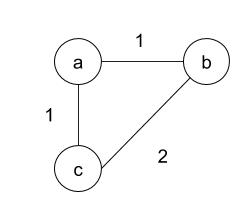
\includegraphics[scale=0.5]{q3}\\
Conversely, if we consider the graph above, there is a unique MST that contains edges $(a,b)$ and $(a,c)$, however the cut $(\{a\}, \{b,c\})$ doesn't have a unique minimum edge crossing the cut.
%Question 4
\newpage
\item \color{blue} Consider a connected graph $G=(V,E)$ where each edge has a non-zero positive weight. Furthermore, assume that all edge weights are distinct.
Using the cut property, first show that that for each vertex $v\in V$, the edge incident to $v$ with
minimum weight belongs to a Minimum Spanning Tree (MST). 
Can you use this to devise an algorithm for MST - the above step identifies at least $|V|/2$ edges in MST - you can collapse these edges, by identifying the vertices and then recursively apply the same technique - the graph in the next step has at most half of the vertices that you started with - and so on. 
What is the running time of your algorithm?\\
Note that for an edge $e=uv$ in the graph $G=(V,E)$, {\em identifying} vertex $u$ with $v$ or {\em collapsing} $e$  is the following operation: Replace the vertices $u$ and $v$  by a new vertex, say $u'$. Remove  the edge between $u$ and $v$.  If there was
an edge from $u$ (respectively, $v$) to any vertex $w$ ($w\not=u$ and $w\not=v$), then we add an edge (with the same weight as of edge  $uw$ (respectively,  $vw$)), between the vertices $u'$ and $w$. This transforms graph $G$ to a new graph $G'=(V',E')$, where $|V'|<|V|$ and $|E'| < |E|$. Note that $G'$ may be a multigraph (i.e., between a pair of vertices, there may be more than one edge). For example, if $uv$,  $uw$,  and  $vw$ are edges in $G$, then $G'$ will have two edges between $u'$ and $w$ when we identify $u$ with $v$. We can transform $G'$ to a simple graph by  keeping  the edge with the lower weight among $uw$ and $vw$ as the representative for $u'w$ for the computation of MST.

\color{black}
\textbf{Solution} 

Assume that {$X \subseteq T$} and $T$ is some MST of  G. We make a cut $(S, V-S)$ that respects $X$. Let's assume that $S = (\{v\})$ where {$v \in V$}, then the cut we make is  $(\{v\}, \{V-v\})$. Let $e$ be the minimum weighted edge crossing the cut. By cuts property, edge $e$ belongs to an MST of G.

\begin{algorithm}
\caption{Finding MST}
\begin{algorithmic}[1]
\Procedure{MST}{$G$}
	\State $F \gets G.V$ \Comment{Initialize F as a set of one-vertex trees, one for each vertex of the graph}

	\While{$F$ has more than 1 component}
		\State Determine the connected components of $F$ and label each vertex of $G$ by its component
		\State Initialize the minEdge for each component of $F$ to be $\infty$
		\For{each edge($u$, $v$) in $G$}
			\If{$ComponentLabel(u) \neq ComponentLabel(v)$ }
				
				\If{$edge(u,v) <$ the minEdge of component of  $u$ }
					\State Set $edge(u,v)$ as minEdge for the component of $u$
				\EndIf
				\If{$edge(u,v) <$ the minEdge of component of  $v$ }
					\State Set $edge(u,v)$ as minEdge for the component of $v$
				\EndIf
			\EndIf
		\EndFor
		\For{each component in $F$}
				\State Add minEdge(component) to $F$
		\EndFor			
	\EndWhile

	\State Return $F$
\EndProcedure
\end{algorithmic}
\end{algorithm}

\textbf{Proof of Correctness}\\
Earlier we proved that that for each vertex $v \in V$, the edge incident to $v$ with minimum weight belongs to a minimum spanning tree. The algorithm above builds upon this idea. We start off with a set of components, one vertex for each component of the graph which is seen on line 2. Inside the while loop, we first determine all the connected components, then for each connected component we find the minimum edge incident to. This while loop terminates once we have only 1 component, and this component is therefore an MST for G. 

\textbf{Time Complexity Analysis}
The initialization of $F$ on line 2 takes O(V) time. The while loop on line 3 will loop $log(V)$ times because the size of the components is at worst case halved each time. The inner for loop  runs $E$ times so the total running time for the for loop takes $O(E$ $logV)$. Therefore the final time complexity for this algorithm is $O(E$ $logV)$.
%Question 5
\item \color{blue} Suppose you are given a set $S$ of $n$ distinct points in the plane.   Let $A$ and $B$ represents a partition of $S$, i.e. $A\subset S$, $B\subset S$, $S=A\cup B$, and $A\cap B=\emptyset$. Define the distance between $A$ and $B$, denoted by  $d(A,B)$, as the minimum among Euclidean distances between pair of points, where one point is from  $A$ and the other from $B$, i.e. 
$$d(A,B)=\min_{a\in A, b\in B}|ab|$$  
Our task here is to find a partition of $S$ into two non-empty sets $A$ and $B$ that maximizes $d(A,B)$. For this, we define a complete graph $G=(V,E)$ on $n$ vertices and ${n\choose 2}$ edges on these points as follows. Each vertex in $V$ represents a distinct point of $S$, and there is an edge between every pair of (distinct) vertices, where the weight of an edge 
$e=(u,v)$ is Euclidean distance between the points corresponding to $u$ and $v$. Consider a minimum spanning tree $T$ of $G$. Let $e$ be the most expensive edge in $T$ (i.e. $e$ is the last edge added to $T$ by Kruskal's algorithm). Let $V_1$ and $V_2$ be the two sets of vertices in the connected components obtained after the removal of $e$ from $T$. Show that the points  corresponding to $V_1$ and $V_2$ forms the required partitioning of $S$.       (Recall that Euclidean distance between  two points  $a=(3,5)$ and $b=(4,2)$ is $|ab|=\sqrt{(3-4)^2+(5-2)^2}= \sqrt{10}$.) 

\color{black}
\textbf{Solution} 

Let's assume edge $e$ is the last edge added to $T$, an MST of $G$, by Kruskal's algorithm and the removal of edge $e$ gives two vertex sets $A$ and $B$ which maximizes $d(A,B)$. Let's assume a contradiction that there is an edge $e'$ that satisfies $d(A',B')$ where $A'$ and $B'$ is some vertex set and $d(A',B') > d(A,B)$. We know that Kruskal's algorithm adds edges that are part of an MST in non-decreasing order and edge $e$ is the last edge added to $T$ to form an MST. So then, we know that there must be some edge in $T$ that crosses $A'$ and $B'$ and this edge will be called $e''$, which causes a contradiction. This is because we said earlier that $d(A',B') > d(A,B)$, or for simplicity, the weight of $e' > e$. However, we know that $e'', e \in T$ and $e$ is added last in $T$, this means $e''\leq e$ and so $e'' <e'$. Therefore, $d(A',B') \leq d(A,B)$ and so the last edge added in Kruskal's algorithm, $e$, maximizes the distance.

%Question 6
\item \color{blue} Let $G=(V,E)$ be a connected simple graph, where each edge has a weight of $3$. Devise an algorithm, running in $O(|V|+|E|)$ time, for computing shortest path distances from a specific vertex $s\in V$ to all other vertices of $G$. 

\color{black}
\textbf{Solution}
\begin{algorithm}
\caption{Shortest path distances from $s$ to all other vertices}
\begin{algorithmic}[1]
\Procedure{SSD}{$G, s$}
	\State $BFS(G,S)$ \Comment{breadth-first search G, starting at s, labelling the depth for each vertex}
	
	\For{each vertex $v \in G.V$}
		\State $\partial(s,v) \gets v.depth * 3$ 
	
	\EndFor 
\EndProcedure
\end{algorithmic}
\end{algorithm}

\textbf{Proof of Correctness}\\
Because each edge weight is the same, 3, we can use breadth first search (BFS) to find all the shortest paths from a specific vertex to all other vertices in G. We know this because the shortest path between two vertices is always the one with the fewest edges required to have a path between them as all edges have the same weight, and so the shortest path distance is defined by the depth of the vertex from the source in a BFS times 3 and this algorithm does exactly that. Therefore this algorithm is correct.\\
\textbf{Time Complexity Analysis}\\
The time complexity of this algorithm is $O(V+E)$ because we visit each vertice and edge once.

%Question 7
\item\color{blue} Prove that the distance values extracted from the heap (priority queue) over the entire execution of Dijkstra's single source shortest path algorithm, in a directed connected graph with positive edge weights, is a NON-Decreasing 
sequence.  Where is this fact used in the correctness of the algorithm?

\color{black}\textbf{Solution}
Referring to the class notes on Dijkstra's single shortest path algorithm, let {$u \in Q$} with minimum $d(u)$ value in an iteration of the while-loop. Before the for-loop is executed, $d(u) \leq d(v)$ for all vertices in $Q$ as $d(u)$ is selected as the minimum. We see that in the for-loop, some of the $d(v)$ values may decrease from its current value to $d(v) = d(u) + weight(edge(u,v)) \geq d(u)$. So we know that $d(v) \geq d(u)$ for all $v \in Q$. This proves the claim 3 that the minimum d-value in $Q$ never decreases and as such the distance values in the heap over the entire execution of Dijkstra's single source shortest path algorithm is  a non-decreasing sequence.  This fact is used for each iteration in $v_1, v_2, ... , v_k$ to show that we keep the vertex that is larger than the previous vertex in the queue, $Q$. For example in $v_1$, we see that $d(v_2)>d(v_1)$, so therefore $v_2 \in Q$.

%Question 8
\item \color{blue}In the summer vacation, you decided to travel to various communities in Northern Canada by your favorite ATV (All-Terrain Vehicle).
%Assume that your chosen ATV can travel on all types of terrain (including lakes/swamp/ice/fly!). 
Each of the communities you want to visit is
represented as a vertex in your travel graph (a total of $|V|$ communities). Moreover, you are provided with distances between  all pairs of  communities. Think of your input graph as a complete graph (i.e. every pair of vertices are joined by an edge), and the weight of an edge, say $e=(uv)$ is the distance
between the community $u$ and $v$. Since this is in far North, and the routes between communities are not used that often, the gas stations 
are only located in communities (there are absolutely no gas stations which are outside a community). Furthermore, we can assume
that each community has at least one gas station. Once you completely fill up the tank of your ATV, it has an upper limit, say of $\Delta$ kilometers, which it can travel, and to travel any further it needs to fill up (which means at that point it needs to be in a community!).
You need to answer the following two questions

\begin{enumerate}
\item First design a method, running in $O(|V|+|E|)$ time, which can answer whether is there some path which your ATV can take, so that 
you can travel between two particular communities, say $s$ and $t$. It is obvious that if the distance between $s$ and $t$ is at most $\Delta$, then you can travel directly without refuelling. Otherwise, you can travel between $s$ and $t$, provided there are communities where we can
refuel and proceed. [For fun you may like to see whether you can travel from La Loche (in Sask.) to Mandorah (in Northen Territories), when your ATV with full tank can travel at most 100 Kms.]
\newpage
\color{black}
\textbf{Solution}
\begin{algorithm}
\caption{Finding a suitable path between $s$ and $t$}
\begin{algorithmic}[1]
\Procedure{BFS}{$G, s, t, limit$} \Comment{limit denotes the ATV's upper limit it can travel}
	\State {Let G' be the same graph as G but with edges that are $\leq$ $limit$}
	
	\State DFS(G', s) \Comment{this labels the pre and post numbers for all vertices starting with s }
	
	\If{$s.pre\leq t.pre$ and $t.post \leq s.post$ }
		\State Return True
	\EndIf
	
	\State Return False
\EndProcedure
\end{algorithmic}
\end{algorithm}

\textbf{Proof of Correctness}
\\We assume that the DFS() algorithm is correct in that it will perform a depth-first search on graph G, starting on vertex s, and label all the pre and post values for each vertex. This algorithm begins by creating a new graph, $G'$, with the same verticies as $G$, but with edges that are $\leq limit$. This way, we know that all edges in $G'$ can be travelled on for the ATV. Then, we perform a DFS() on $G'$ starting on $s$. We know that in order for there to be a path between $s$ and $t$, the pre and post numbers for $s$ must encompass the pre and post numbers for $t$. This means that {$s.pre\leq t.pre$ and $t.post \leq s.post$ } and this is exactly what line 4 checks for. Therefore this algorithm is correct.

\textbf{Time Complexity Analysis}
\\Line 2 takes $O(V+E)$, line 3 takes $O(V+E)$ and the rest takes constant time. So this algorithm as an overal run time of $O(V+E)$

\newpage
\item \color{blue}Design an algorithm running in $O(|E|\log |V|)$ time to determine the smallest value of $\Delta$, which will enable you to travel from $s$ to $t$. (Please present Pseudocode, correctness, analysis) and use the algorithms discussed in the class/book as black boxes).
\\
\color{black}
\textbf{Solution}
\begin{algorithm}
\caption{Finding a smallest upper limit}
\begin{algorithmic}[1]
\Procedure{SmallestBottleneck}{$G, s, t$}  \Comment{A modification to Dijkstra's algorithm, refer to class notes}
	\For{$v \in V$}
		\State $bottleneck(v) \gets \infty$
	\EndFor
	
	\State $bottleneck(s) \gets 0$; $S \gets \emptyset$; $Q \gets G.V$
	\While{$Q \neq \emptyset$}
		\State $u \gets$ {\em Extract-Min(Q)}
		\State DELETE $u$ from $Q$
		\State INSERT $u$ in $S$
		\For{ each vertex $v$ such that $(u,v) \in E$}
			\If{$bottleneck(u) < wt(u,v)$}
				\State $bottleneck(v) \gets MIN(bottleneck(v),wt(u,v))$
			\Else
				\State $bottleneck(v) \gets MIN(bottleneck(u),bottleneck(v))$
			\EndIf
		\EndFor
	\EndWhile
	\State Return $bottleneck(t)$
\EndProcedure
\end{algorithmic}
\end{algorithm}

\textbf{Proof of Correctness}
\\The algorithm is a slight modification to Dijkstra's algorithm. We see that everything is the same other than instead of keeping track of the shortest path distance for each vertex, we keep track of the smallest bottleneck path for each vertex. So, like how we proved the correctness of Dijkstra's algorithm for single shortest path distance, the same proof can be applied for this algorithm as well.
The modified lines are in the for loop, line 10-13. We see here for each $v$ such that the edge $(u,v)\in E$, we first check if the previous bottleneck in the path which is  $bottleneck(u)$ is smaller than the incoming weighted edge, $wt(u,v)$, to $v$. If that is the case, then we know that the bottleneck for $v$ must be the minimum between it's current bottleneck value and the $wt(u,v)$. Otherwise if the incoming weight is smaller than $bottleneck(u)$, we take the minimum between $bottleneck(v)$ and $bottleneck(u)$. From this, we can see that the claims made in the proof for Dijkistra's algorithm can be made here and the rest can follow. Therefore this algorithm is correct.

\textbf{Time Complexity Analysis}
\\The running time for Dijkstra's algorithm is $O(E $ $Log (V))$


\end{enumerate}

\end{enumerate}

\end{document}